\section{Vorbereitung}
\label{sec:Vorbereitung}
Es wird für 10 Abstände $r$ zwischen 5 und 25\,cm das Drehmoment auf eine Stange berechnet. 
Einmal wird die Kraft im rechten Winkel angesetzt, einmal im 45°-Winkel. \\
\noindent
In Tabelle \ref{tab:Vorbereitung} sind die errechneten Werte aufgeführt.
\begin{figure}
    \begin{minipage}{0.39\textwidth}
    \begin{align*} 
    \intertext{Senkrecht:}
    \vec M&=\begin{pmatrix} 0\\F\end{pmatrix}\times
    \begin{pmatrix} r\\0\end{pmatrix}=F\cdot r\cdot\begin{pmatrix} 1\\-1\end{pmatrix}\\
    \Rightarrow |\vec M|&=F\cdot r
    \intertext{45°-Winkel:}
    \vec M&=\begin{pmatrix} \cos(\varphi F)\\ \sin(\varphi F)\end{pmatrix}
    \times \begin{pmatrix} r\\0 \end{pmatrix}\\
    &=\begin{pmatrix} 
    \phantom{-}r\cdot F\cdot\sin(\varphi)\\ -r\cdot F\cdot\sin(\varphi)\end{pmatrix}\\
    \Rightarrow |\vec M|&=Fr\cdot\sin(\varphi)
    \end{align*}
    \end{minipage}
    \hfill
    \begin{minipage}{0.28\textwidth}
        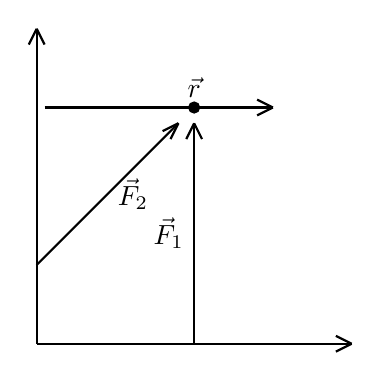
\begin{tikzpicture}
            \centering
            % Koordinatensystem
            \draw[thick] (0,0) -- (0,4);
            \draw[thick] (0,0) -- (4,0);
            \draw[thick] (0,4) -- (-0.1,3.8);
            \draw[thick] (0,4) -- (0.1,3.8);
            \draw[thick] (4,0) -- (3.8,0.1);
            \draw[thick] (4,0) -- (3.8,-0.1);
            % r
            \filldraw[black] (2,3) node[above] {$\vec r$} circle (2pt);
            % Stange
            \draw[thick] (0.1,3) -- (3,3);
            \draw[thick] (3,3) -- (2.8,3.1);
            \draw[thick] (3,3) -- (2.8,2.9);
            % F_1
            \draw[thick] (2,0) -- node[left] {$\vec F_1$} (2,2.8);
            \draw[thick] (2,2.8) -- (1.9,2.6);
            \draw[thick] (2,2.8) -- (2.1,2.6);
            % F_2
            \draw[thick] (0,1) -- node[right] {$\vec F_2$} (1.8,2.8);
            \draw[thick] (1.8,2.8) -- (1.6,2.7);
            \draw[thick] (1.8,2.8) -- (1.7,2.6);
            \end{tikzpicture}
    \end{minipage}
    \begin{minipage}{0.27\textwidth}
        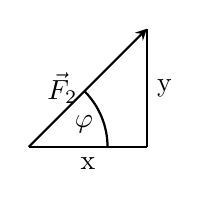
\begin{tikzpicture}
        \draw[thick,-stealth] (1,0) --node[left]{$\vec F_2$} (2.5,1.5);
        \draw[thick] (1,0) -- node[below] {x} (2.5,0);
        \draw[thick] (2.5,0) -- node[right] {y} (2.5,1.5);
        \draw[thick] (2,0) arc (0:45:1);
        \draw (1.7,0.29) node {$\varphi$};
        \end{tikzpicture}
        \begin{align*}
            \sin(\varphi)&=\frac{y}{|\vec F_2|}\\
            \cos(\varphi)&=\frac{x}{|\vec F_2|}
        \end{align*}
    \end{minipage}
\end{figure}
\begin{table}
    \centering
    \caption{Drehmoment für zwei verschiedene Winkel und zehn verschiedene Radien 
    und eine Kraft von $\SI{0.1}{\newton}$.}
    \label{tab:Vorbereitung}
    \begin{tblr}{colspec={c | c c }}
    \toprule
    $r$ / cm & M für $\vec F \perp \vec r$ / J & M für $\angle(\vec r, \vec F)=45°$ / J\\ 
    \midrule
    5  & 0,5 & 0,35\\
    7  & 0,7 & 0,49\\
    9  & 0,9 & 0,63\\
    11 & 1,1 & 0,78\\
    13 & 1,3 & 0,92\\
    15 & 1,5 & 1,06\\
    17 & 1,7 & 1,20\\
    19 & 1,9 & 1,34\\
    21 & 2,1 & 1,48\\
    23 & 2,3 & 1,63\\
    25 & 2,5 & 1,77\\
    \bottomrule
    \end{tblr}
\end{table}